%% 
%% Copyright 2007, 2008, 2009 Elsevier Ltd
%% 
%% This file is part of the 'Elsarticle Bundle'.
%% ---------------------------------------------
%% 
%% It may be distributed under the conditions of the LaTeX Project Public
%% License, either version 1.2 of this license or (at your option) any
%% later version.  The latest version of this license is in
%%    http://www.latex-project.org/lppl.txt
%% and version 1.2 or later is part of all distributions of LaTeX
%% version 1999/12/01 or later.
%% 
%% The list of all files belonging to the 'Elsarticle Bundle' is
%% given in the file `manifest.txt'.
%% 
%% Template article for Elsevier's document class `elsarticle'
%% with harvard style bibliographic references
%% SP 2008/03/01

%\documentclass[preprint,12pt,authoryear]{elsarticle}

%% Use the option review to obtain double line spacing
%% \documentclass[authoryear,preprint,review,12pt]{elsarticle}

%% Use the options 1p,twocolumn; 3p; 3p,twocolumn; 5p; or 5p,twocolumn
%% for a journal layout:
%% \documentclass[final,1p,times,authoryear]{elsarticle}
%\documentclass[final,1p,times,twocolumn,authoryear]{elsarticle}
%% \documentclass[final,3p,times,authoryear]{elsarticle}
%\documentclass[final,3p,times,twocolumn,authoryear]{elsarticle}
%% \documentclass[final,5p,times,authoryear]{elsarticle}

\documentclass[final,5p,times,twocolumn,authoryear]{elsarticle}

%% For including figures, graphicx.sty has been loaded in
%% elsarticle.cls. If you prefer to use the old commands
%% please give \usepackage{epsfig}

%% The amssymb package provides various useful mathematical symbols
\usepackage{amssymb}
\usepackage{array}
\usepackage{biblatex}

\usepackage{graphicx}
\usepackage{placeins}

\usepackage{xpatch}
% \usepackage{biblatex}

\usepackage{etoolbox,lipsum}
\makeatletter
\patchcmd\@maketitle\@author{\@author \\[\normalbaselineskip] \myfigure}{}{}
\newcommand\myfigure{%
  \makebox[0pt]{
 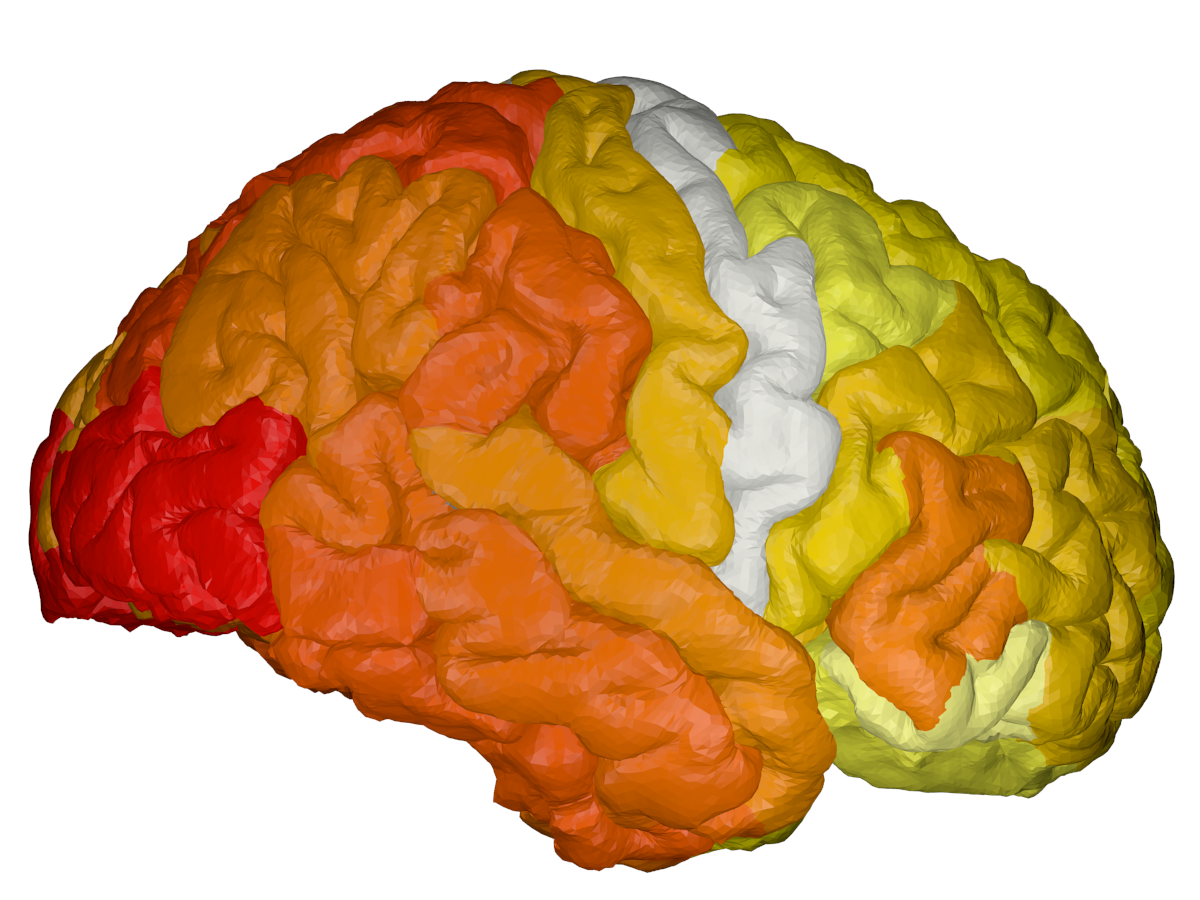
\includegraphics[height=3cm]{images/cortical-front_0.png}
 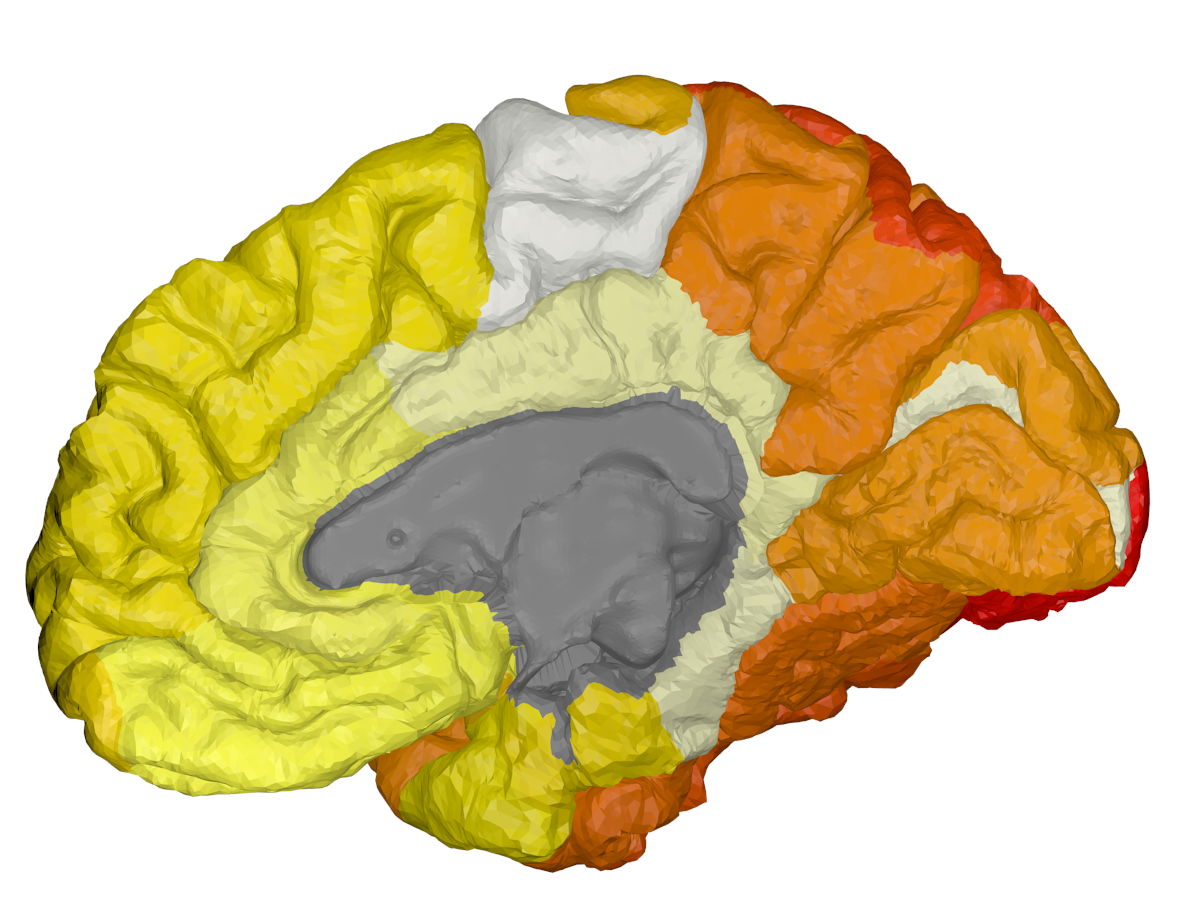
\includegraphics[height=3cm]{images/cortical-back_0.png}
 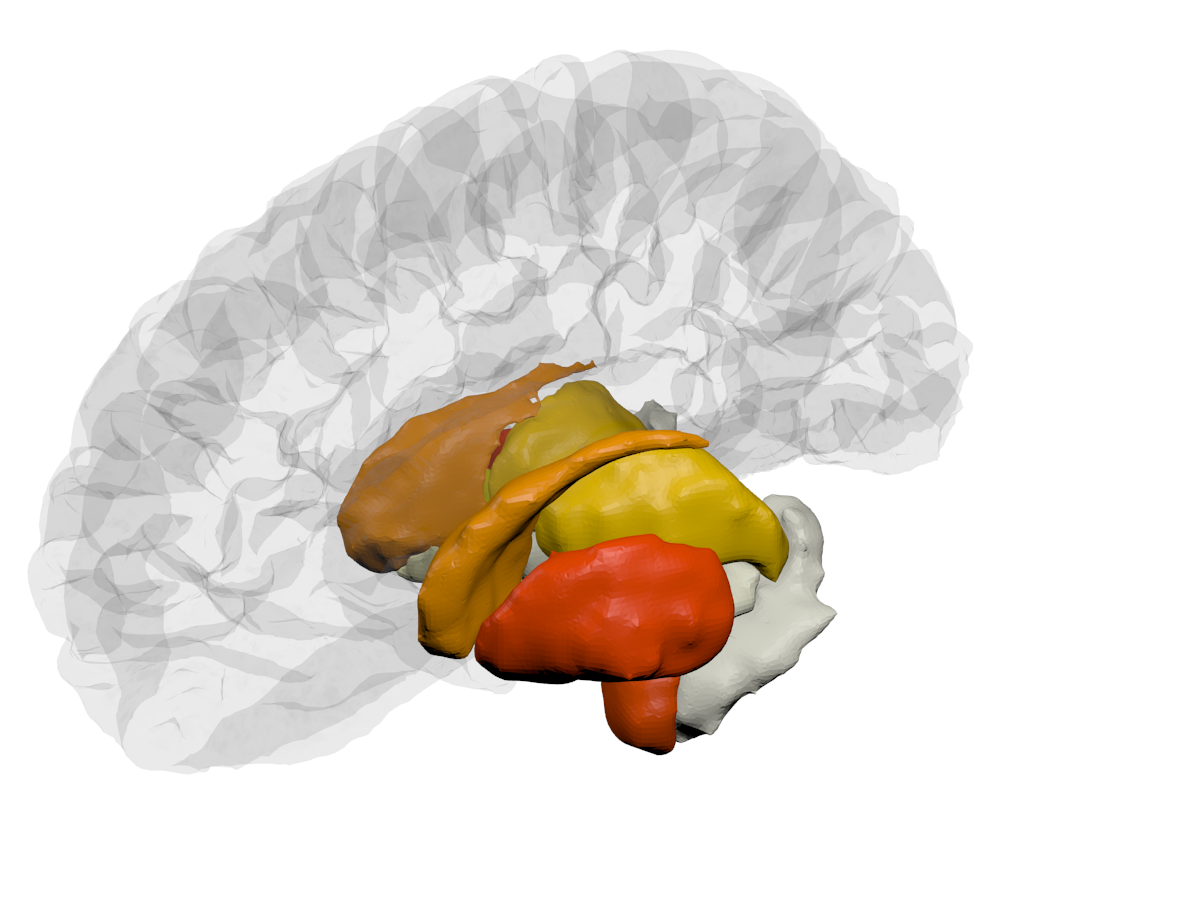
\includegraphics[height=3cm]{images/subcortical_0.png}
} \\[\normalbaselineskip]
  \refstepcounter{figure}\normalfont\textbf{Figure~\thefigure: Some stuff about the teaser}
  \label{fig-teaser}
}
\makeatother


\usepackage[font=normalfont,labelfont=bf]{caption}

%% The amsthm package provides extended theorem environments
%% \usepackage{amsthm}

%% The lineno packages adds line numbers. Start line numbering with
%% \begin{linenumbers}, end it with \end{linenumbers}. Or switch it on
%% for the whole article with \linenumbers.
%% \usepackage{lineno}



\usepackage{etoolbox}
% \patchcmd{<cmd>}{<search>}{<replace>}{<success>}{<failure>}
\patchcmd{\emailauthor}{(#2)}{}{}{}
\patchcmd{\urlauthor}{(#2)}{}{}{}

\journal{}

\makeatletter
\def\ps@pprintTitle{%
 \let\@oddhead\@empty
 \let\@evenhead\@empty
 \def\@oddfoot{}%
 \let\@evenfoot\@oddfoot
 }
\makeatother

\usepackage{xcolor}


\usepackage{hyperref}
\definecolor{links}{HTML}{01368e}
% \hypersetup{colorlinks,linkcolor=links,urlcolor=links}

\makeatletter
\hypersetup{colorlinks=true}
\AtBeginDocument{\@ifpackageloaded{hyperref}
  {\def\@linkcolor{links}
   \def\@anchorcolor{links}
   \def\@citecolor{links}
   \def\@filecolor{links}
   \def\@urlcolor{links}
   \def\@menucolor{links}
   \def\@pagecolor{links}
\begingroup
  \@makeother\`%
  \@makeother\=%
  \edef\x{%
    \edef\noexpand\x{%
      \endgroup
      \noexpand\toks@{%
        \catcode 96=\noexpand\the\catcode`\noexpand\`\relax
        \catcode 61=\noexpand\the\catcode`\noexpand\=\relax
      }%
    }%
    \noexpand\x
  }%
\x
\@makeother\`
\@makeother\=
}{}}
\makeatother


\usepackage{filecontents}

\begin{filecontents*}{bibliography.bib}
@article{jack2010hypothetical,
  title={Hypothetical model of dynamic biomarkers of the Alzheimer's pathological cascade},
  author={Jack Jr, Clifford R and Knopman, David S and Jagust, William J and Shaw, Leslie M and Aisen, Paul S and Weiner, Michael W and Petersen, Ronald C and Trojanowski, John Q},
  journal={The Lancet Neurology},
  volume={9},
  number={1},
  pages={119--128},
  year={2010},
  publisher={Elsevier}
}
@article{scahill2002mapping,
  title={Mapping the evolution of regional atrophy in Alzheimer's disease: unbiased analysis of fluid-registered serial MRI},
  author={Scahill, Rachael I and Schott, Jonathan M and Stevens, John M and Rossor, Martin N and Fox, Nick C},
  journal={Proceedings of the National Academy of Sciences},
  volume={99},
  number={7},
  pages={4703--4707},
  year={2002},
  publisher={National Acad Sciences}
}
@article{seeley2009neurodegenerative,
  title={Neurodegenerative diseases target large-scale human brain networks},
  author={Seeley, William W and Crawford, Richard K and Zhou, Juan and Miller, Bruce L and Greicius, Michael D},
  journal={Neuron},
  volume={62},
  number={1},
  pages={42--52},
  year={2009},
  publisher={Elsevier}
}
@article{migliaccio2015mapping,
  title={Mapping the progression of atrophy in early-and late-onset Alzheimer’s disease},
  author={Migliaccio, Raffaella and Agosta, Federica and Possin, Katherine L and Canu, Elisa and Filippi, Massimo and Rabinovici, Gil D and Rosen, Howard J and Miller, Bruce L and Gorno-Tempini, Maria Luisa},
  journal={Journal of Alzheimer's Disease},
  volume={46},
  number={2},
  pages={351--364},
  year={2015},
  publisher={IOS Press}
}
@article{chard2002brain,
  title={Brain atrophy in clinically early relapsing--remitting multiple sclerosis},
  author={Chard, DT and Griffin, CM and Parker, GJM and Kapoor, R and Thompson, AJ and Miller, DH},
  journal={Brain},
  volume={125},
  number={2},
  pages={327--337},
  year={2002},
  publisher={Oxford University Press}
}
@article{schoonheim2012subcortical,
  title={Subcortical atrophy and cognition: sex effects in multiple sclerosis},
  author={Schoonheim, Menno M and Popescu, Veronica and Lopes, Fernanda C Rueda and Wiebenga, Oliver T and Vrenken, Hugo and Douw, Linda and Polman, Chris H and Geurts, Jeroen JG and Barkhof, Frederik},
  journal={Neurology},
  volume={79},
  number={17},
  pages={1754--1761},
  year={2012},
  publisher={AAN Enterprises}
}
@article{mak2014subcortical,
  title={Subcortical atrophy is associated with cognitive impairment in mild Parkinson disease: a combined investigation of volumetric changes, cortical thickness, and vertex-based shape analysis},
  author={Mak, E and Bergsland, N and Dwyer, MG and Zivadinov, R and Kandiah, N},
  journal={American Journal of Neuroradiology},
  volume={35},
  number={12},
  pages={2257--2264},
  year={2014},
  publisher={Am Soc Neuroradiology}
}
@article{coughlin2015neuroinflammation,
  title={Neuroinflammation and brain atrophy in former NFL players: an in vivo multimodal imaging pilot study},
  author={Coughlin, Jennifer M and Wang, Yuchuan and Munro, Cynthia A and Ma, Shuangchao and Yue, Chen and Chen, Shaojie and Airan, Raag and Kim, Pearl K and Adams, Ashley V and Garcia, Cinthya and others},
  journal={Neurobiology of disease},
  volume={74},
  pages={58--65},
  year={2015},
  publisher={Elsevier}
}
@inproceedings{pieper20043d,
  title={3D Slicer},
  author={Pieper, Steve and Halle, Michael and Kikinis, Ron},
  booktitle={2004 2nd IEEE international symposium on biomedical imaging: nano to macro (IEEE Cat No. 04EX821)},
  pages={632--635},
  year={2004},
  organization={IEEE}
}
@article{fischl2012freesurfer,
  title={FreeSurfer},
  author={Fischl, Bruce},
  journal={Neuroimage},
  volume={62},
  number={2},
  pages={774--781},
  year={2012},
  publisher={Elsevier}
}
@book{penny2011statistical,
  title={Statistical parametric mapping: the analysis of functional brain images},
  author={Penny, William D and Friston, Karl J and Ashburner, John T and Kiebel, Stefan J and Nichols, Thomas E},
  year={2011},
  publisher={Elsevier}
}
\end{filecontents*}

% \addbibresource{bibliography.bib}

\usepackage{natbib}
\usepackage{tikz}

\begin{document}


\begin{frontmatter}

\title{BrainPainter: A software for the visualisation of brain structures, biomarkers and associated pathological processes}

\ead{razvan@csail.mit.edu}
\ead[url]{https://github.com/mrazvan22/brain-coloring}

\address[mit]{Computer Science and Artificial Intelligence Laboratory, Massachusetts Institute of Technology, Cambridge, USA, MA 02139}
\address[ucl]{Centre for Medical Image Computing, University College London, Gower Street, London, United Kingdom, WC1E 6BT}

\author[mit,ucl]{R\u{a}zvan V. Marinescu}
\author[ucl]{Daniel C. Alexander}
\author[mit]{Polina Golland}

% \begin{abstract}
% 
% \end{abstract}

% \begin{keyword}
% Brain visualisation \sep
% Neurodegenerative diseases
% \end{keyword}

\end{frontmatter}


\begin{figure}
\centering

\begin{tikzpicture}
    \node (A) at (0,1.5) {\textbf{INPUT}};
\node (A2) at (0,0) {\begin{tabular}{c | c c c c}
 Biomarkers &  hippocampus & inferior & superior & ...\\
  &   & temporal & parietal & ...\\
  \hline
Brain 1 & 0.6 & 2.3 & 1.3 & .. \\
Brain 2 & 1.2 & 0.0 & 3.0 & .. \\
... & ...\\
\end{tabular}};
 \node (B) at (0,-3) {\textbf{OUTPUT}};
 \node (C) at (0,-5) {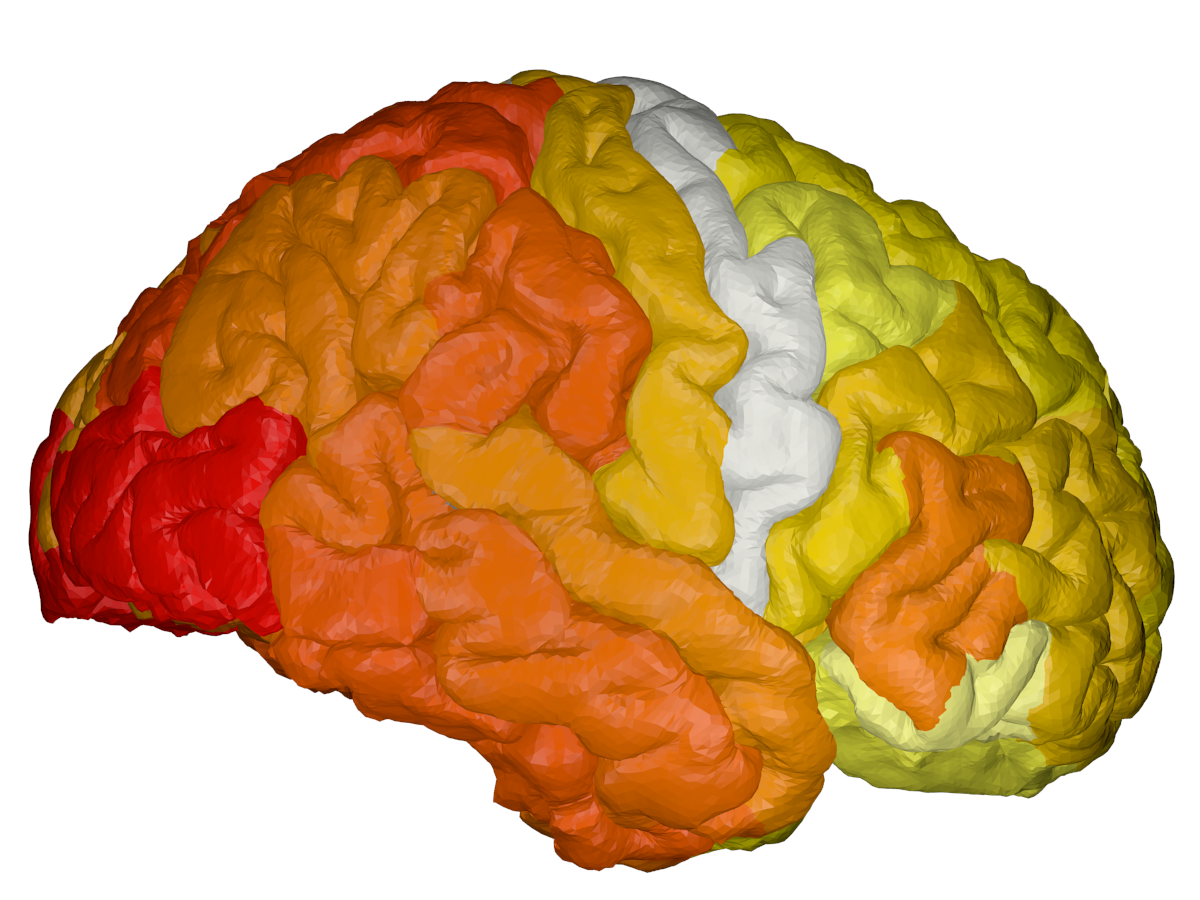
\includegraphics[height=2.3cm]{images/cortical-front_0.png}
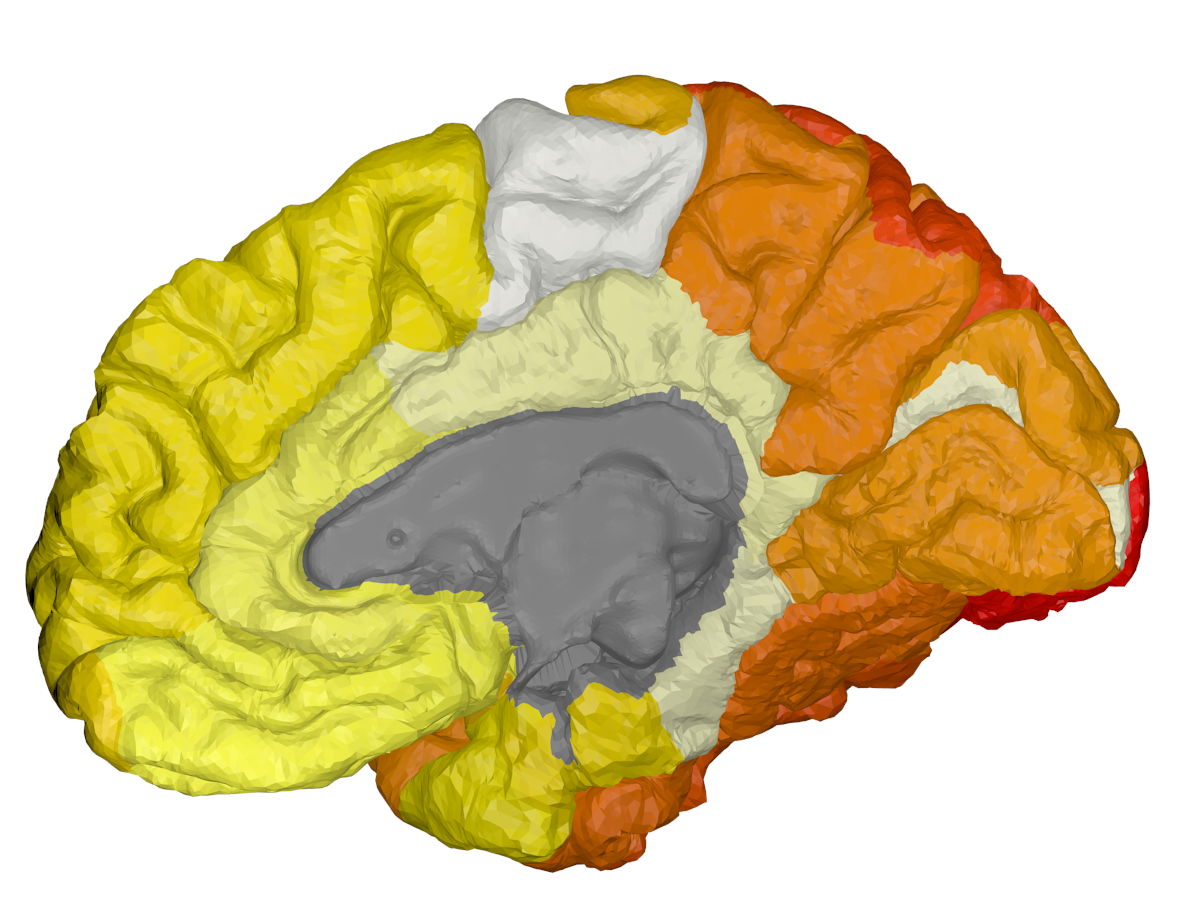
\includegraphics[height=2.3cm]{images/cortical-back_0.png}
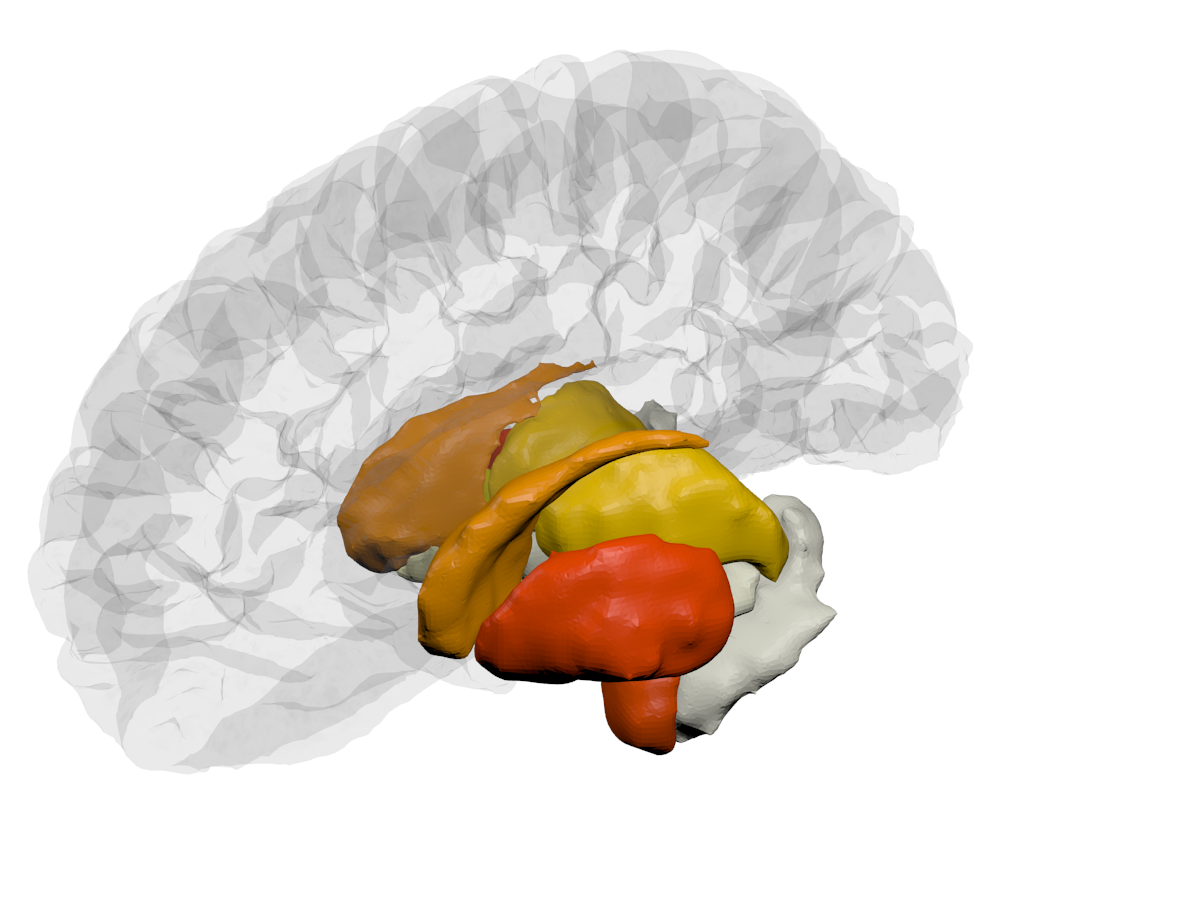
\includegraphics[height=2.3cm]{images/subcortical_0.png}
};
 \node (C2) at (C.north) {Brain 1};

    \node (D) at (0,-8.2) {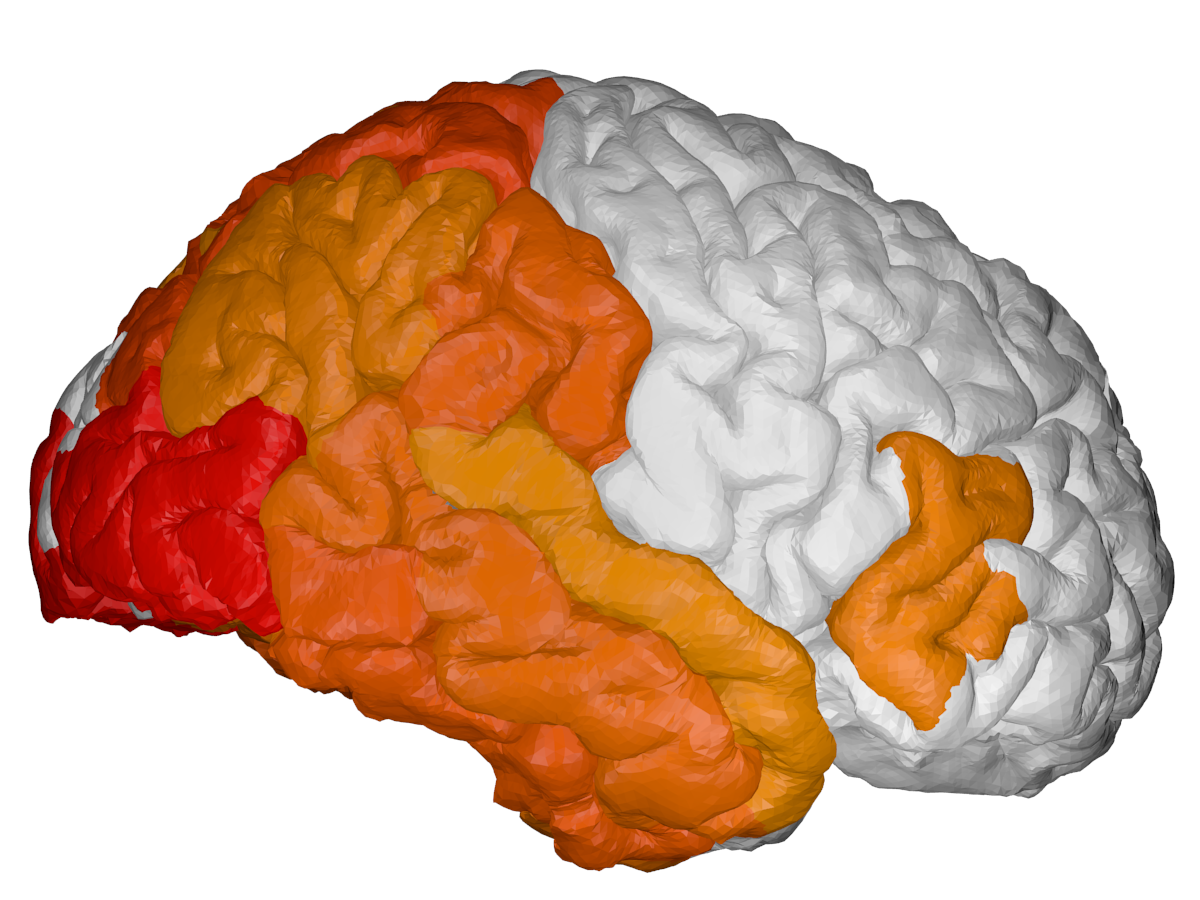
\includegraphics[height=2.3cm]{images/cortical-front_1.png}
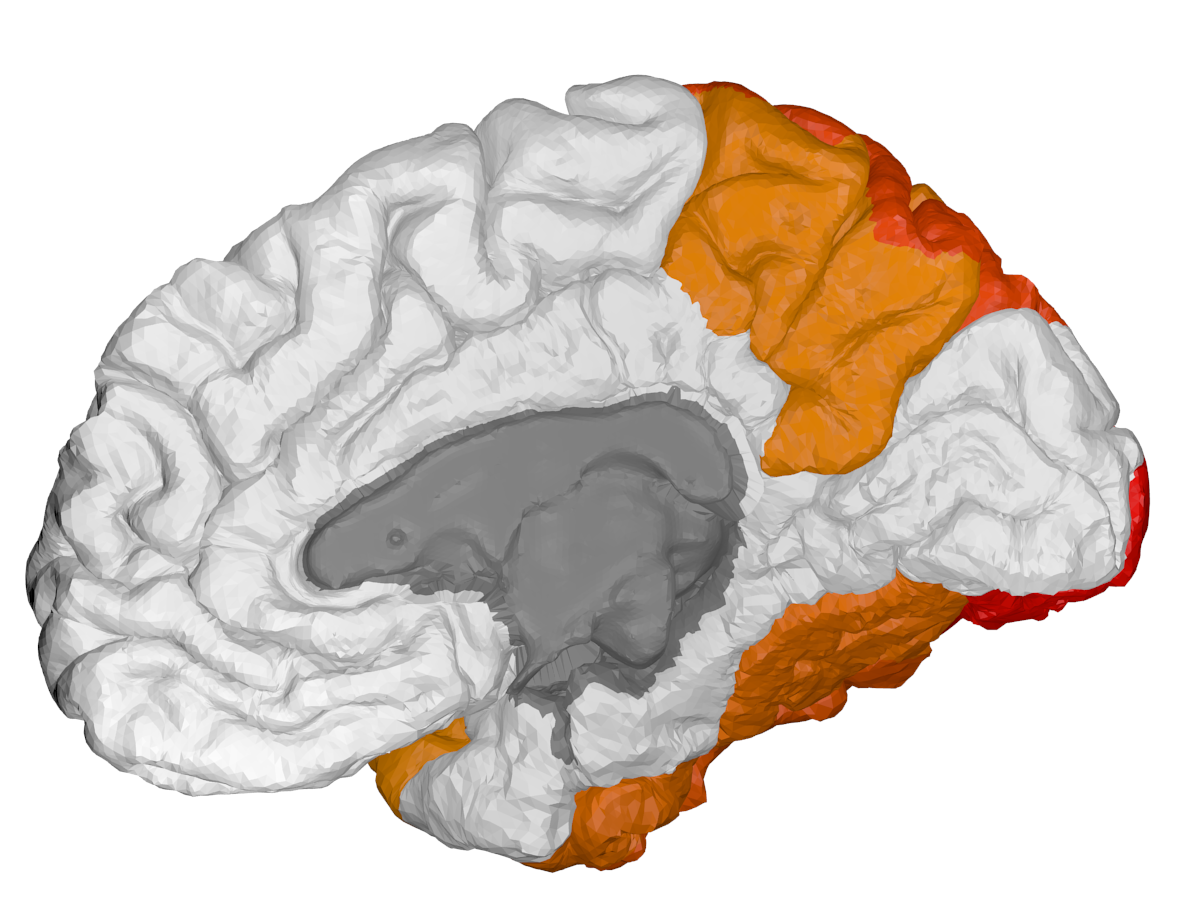
\includegraphics[height=2.3cm]{images/cortical-back_1.png}
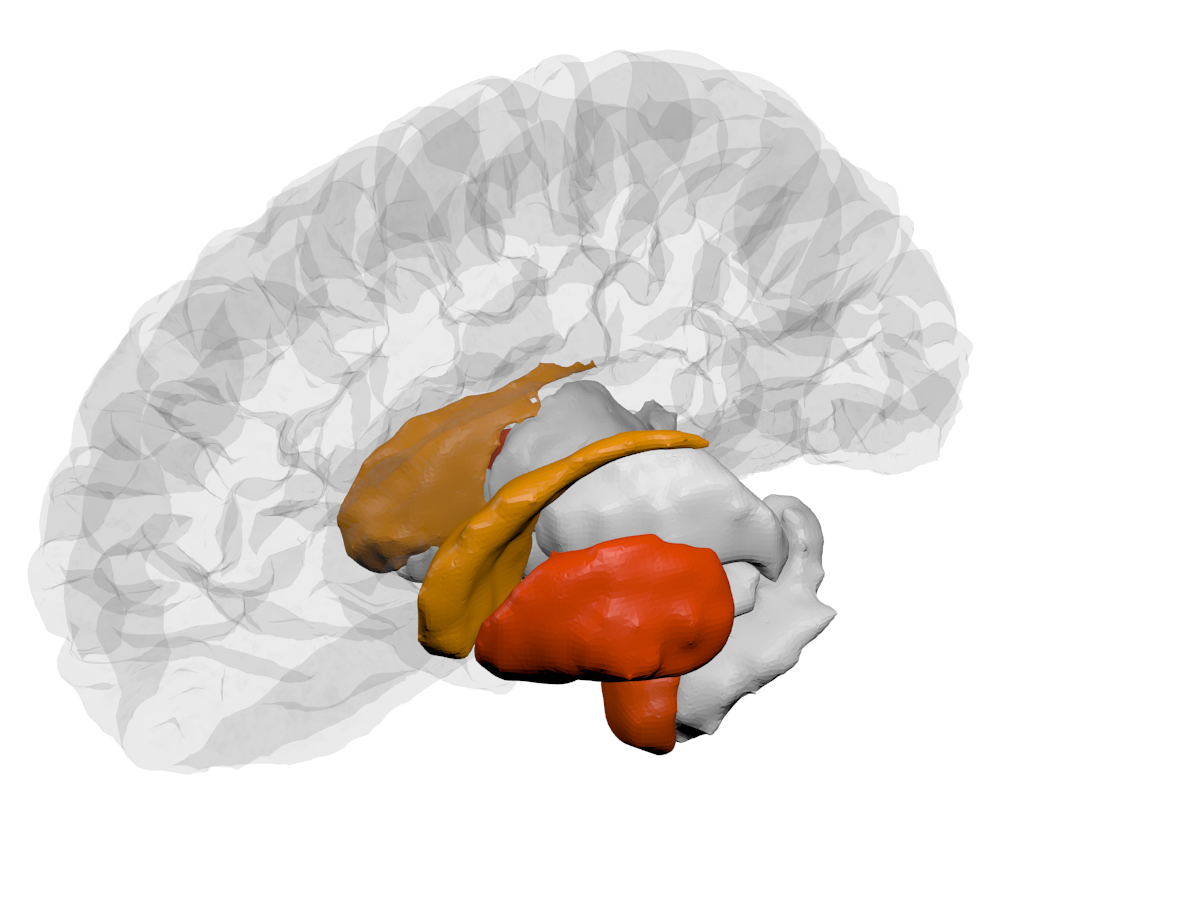
\includegraphics[height=2.3cm]{images/subcortical_1.png}};
 \node (D2) at (D.north) {Brain 2};

    \draw[thick,->] (A2) -- (B) node[midway,left] {\textbf{\large{BrainPainter}}};
  \end{tikzpicture}
\caption{Given a .csv file with biomarkers corresponding to different brain regions, we automatically generate brain images with the cortical surface (left and middle), along with subcortical structures (right).}
\end{figure}


%% \linenumbers

%% main text



% \FloatBarrier

\section*{Abstract}
% \label{intro}

We present BrainPainter, a software that automatically ...


\section{Introduction}
\label{intro}


% diagram showing the aim: input numbers and output images

Visualisation of brain structure, function and pathology is crucial for understanding the mechanisms underlying certain neurodegenerative diseases and eases the interpretation of results in brain medical imaging. This is especially important in populations studies, where two or more populations are compared for any group differences in biomarkers derived from e.g. Magnetic Resonance Imaging, Positron Emmission Tomography (PET) or Computer Tomography (CT). However, for traumatic brain injury or rarer neurodegenerative diseases such as Parkinson's disease or Multiple Sclerosis, the visualisation of statistical results is sometimes not performed due to the inability to register images to a common template or lack of robust registration software, hence many studies  \cite{coughlin2015neuroinflammation,mak2014subcortical,schoonheim2012subcortical,chard2002brain} only report differences between patients and controls in tables or as box plots. 

When alignment to a common population template is possible, e.g. in Alzheimer's disease, excellent 3D visualisation software exists (e.g. 3D slicer \cite{pieper20043d}, Freeview \cite{fischl2012freesurfer} or SPM \cite{penny2011statistical}) which allows interactive visualisation of population differences e.g. the output of voxel-based morphometry (VBM). However, such software have several inherent limitations. First, such software (e.g. Freesurfer\footnote{We actually refer to Freeview, which is the visualisation software bundled with Freesurfer}) generally requires inputs in their own data format, which is usually difficult and time-consuming to create without using their pipeline. Secondly, for highlighting complex patterns of pathology, authors need to show multiple slices from the same 3D image (generally from 4 (\cite{seeley2009neurodegenerative}) up to 8 slices (\cite{migliaccio2015mapping}), which ends up taking too much space on the academic paper being publised. While Freesurfer solves this using a cortical surface-based representation that captures all the complexity of pathology patterns in a single image, it cannot visualise subcortical structures. Third, current software cannot be easily used to generate a movie showing a dynamic process, e.g. propagation of pathology within the human brain.

We present BrainPainter, a software for easy visualisation of structures, pathology and biomarkers in the brain. As opposed to previous visualisation software, the input data is a simple list of numbers in a .csv file representing colours to be assigned to each brain structure. Secondly, it can visualise patterns on both cortical and subcortical structures using a surface repreentation, removing the need to show multiple slices. Third, the images are generated automatically from pre-defined view-points, allowing one to create a movie showing e.g. the propagation of pathology, without the need to write any extra software code. BrainPainter is open source and available on Github: \url{https://github.com/mrazvan22/brain-coloring}.



%\FloatBarrier
\section{Design}
\label{design}

% diagram showing the Design. what kind of atlases can it take, type of colouring, blender integration


BrainPainter works 



\FloatBarrier
\section{Use case: Show progression of pathology}
\label{design}


\section{Conclusion} 




\FloatBarrier
\section{Acknowledgements}




RVM is supported by the EPSRC Centre For Doctoral Training in Medical Imaging with grant EP/L016478/1. NPO, FB, SK, and DCA are supported by EuroPOND, which is an EU Horizon 2020 project. ALY is currently supported by an EPSRC Doctoral Prize fellowship and was previously supported by EPSRC grant EP/J020990/01. DCA is supported by EPSRC grants J020990, M006093 and M020533. Data collection and sharing for this project was funded by the Alzheimer's Disease Neuroimaging Initiative (ADNI) (National Institutes of Health Grant U01 AG024904) and DOD ADNI (Department of Defense award number W81XWH-12-2-0012). FB is supported by the NIHR UCLH biomedical research centre and the AMYPAD project, which has received support from the EU-EFPIA Innovative Medicines Initiatives 2 Joint Undertaking (AMYPAD project, grant 115952). This project has received funding from the EU Horizon 2020 research and innovation programme under grant agreement No 666992.

bibliography
% \appendix





\section*{References}

\bibliographystyle{elsarticle-harv}
\bibliography{bibliography}

% \printbibliography

\xpatchbibmacro{date+extrayear}{%
  \printtext[parens]%
}{%
  \setunit{\addperiod\space}%
  \printtext%
}{}{}

\printbibliography


\end{document}




\endinput


%%
%% End of file `elsarticle-template-harv.tex'.
